\chapter[SCP-042 昔日天马]{
    SCP-042 A Formerly Winged Horse\\
    SCP-042 昔日天马
}

\label{chap:SCP-042}

\begin{figure}[H]
    \centering
    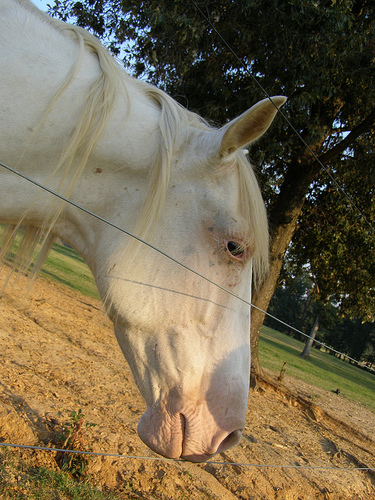
\includegraphics[width=0.5\linewidth]{images/SCP.042.jpg}
    \caption*{SCP-042被用带电护栏逼迫站起时的状态。}
\end{figure}

\bb{项目编号:}SCP-042

\bb{项目等级:}Safe

\bb{特殊收容措施:}SCP-042现被收容于32号生物研究站点(Bio-Research Area-32)的12号最低安全警戒围栏中,尽管SCP-042看起来根本就没有表现出要逃离收容设施的意图,但在其收容措施周围仍应随时保持必要的安全手段。之前进行的试图维持12号围栏中植被活力的尝试到目前为止都失败了。尽管进行了常规的浇水行为,但SCP-042出现并踩踏过的所有土地都会变为焦土。目前为止仍不能确定额外加入的水究竟发生了什么,并且,出于该行为没有成果和有可能对于当地的地下水位产生极大危险的考虑,浇水的计划已经被终止。对于当地水位的检测和水样的分析调查将每周进行一次。

与SCP-042进行互动的人员,包括动物驯养员、医药人员、饲养员以及看守人员,都必须接受一次彻底的搜查,该搜查也要在{[}数据被编辑]以及高级人员进入12号围栏时进行。任何试图夹带武器,或者可以多为武器使用的物品进入围栏的人员将马上被{[}数据被编辑]。以任何方式与SCP-042进行了互动的人员都必须每周接受一次心理测试。所有的对于SCP-042背部伤口进行的医学检查都必须近距离监控以防有人试图对SCP-042进行安乐死。

\bb{描述:}SCP-042是一只被认为是马属的动物,其皮毛为白色并且有着一些棕色的斑点。它站立时脊背高度为183CM(18手),重量达710公斤。因为缺乏运动和拒绝进食引起的萎缩,它的重量自被基金会监管以来已经显著地下降了。尽管现已强行给它灌食流体食物,SCP-042依然十分瘦弱不堪。在SCP-042背上有着2个大型的骨质突起物,并且这2个突起都连接到其背部强有力的肌肉组织之中(现已萎缩)。这2个突起从042背部延伸至其末端的长度为37CM,并且是从SCP-042背部2道锯齿状的开放性伤口处伸出的。这2道伤口到目前为止尚未发现有愈合的迹象,虽然推断其内部应该已经发生了凝血,否则SCP-042早已因失血过多而亡。

SCP-042表现出无精打采的状态并且对所有训练有素的驯兽师进行的煽动性行为都几乎没有反应。如果条件允许,SCP-042将一直趴在地上,不会有任何企图进行饮食或是逃跑的移动行为。痛苦反应测试(Pain-response conditioning)已经证明了存在着某种有效的方法使得SCP-042站起来让它得到清洗,但事实上不管力量冲击有多么强烈,SCP-042总是试图重新躺下,即便是它已经失去了意识也是如此。

在SCP-042的智力水平上研究者们一直存在着分歧,一部分人认为它并不会比与它同属的其他生物更为聪明,但另一部分人认为事实上SCP-042可能是一名智者。已经观察到SCP-042会与进入12号围栏的人员进行目光的接触,这些人员之中的大部分人都把这种目光描述为“恳求”。SCP-042已经在不同的场合之中遭遇了数起事故并受伤,事故的原因从设备的碎片到其收容设施的围墙不一而足。在对于其智力的争论之中这些事故被认为是SCP-042自身有意为之的。

\bb{附录:}P██████博士于█\slash ██\slash 19██提交了一份把SCP-042转移到4号生物研究站点的申请,并已经被O5-5同意。P██████博士改变了运输文档并指示SCP-042应该进行航空运输而不是在陆地上由武装警卫队押运。在运输过程之中,P██████博士制服了飞行员并夺得了运输机的掌控权,使飞机开始了极大角度的快速俯冲,期间乘客和货物都经历了将近一分钟的失重状态直到安全人员重新夺回了飞机的控制权并将飞机平稳下来。在P██████博士被绑起来到飞机降落这段时间内,SCP-042逃离了它的收容措施并且在货舱区踢死了2名安全人员。货舱的安全录像显示在这之后,SCP-042来到了P██████博士身边并且将它的鼻子蹭在了P██████博士的脸上,在这段接触时间内P██████博士表现的十分欣慰。但当增援人员到来用镇静标制服了042并且这段接触被破坏之后,P██████博士陷入了一直不能痊愈的紧张性精神病状态之中,在听到了他的所作所为之后,P██████博士于██\slash ██\slash 19██在接受基金会药物治疗时对自己进行了安乐死。
